\section{Corrections}

When analyzing the data, there are several corrections that need to be made. These are due to various physical or systematic effects that took place during the experiment. These effects have been studied in order to determine a ``correction factor'' that can be applied to the data.

\subsection{Energy Loss}

Incoming and outgoing electrons lose energy due to passing through target material. This energy loss occurs due to the electrons striking electrons in the atoms of the target and the surrounding material. This calculation is done inside of the replay code for the experiment. The calculation assumes that the scattering occurs at the center of the target. The air gap, upstream endcap, and target material through half of the target length is used to calculate the energy loss for the incoming electron. Using the scattering angle, the target material, cell wall, scattering chamber wall, and outgoing air gap are used to calculate the energy loss for the scattered electron. This calculation is done using the Bethe-Bloch stopping-power formula as described in \cite{eloss}.

\subsection{Computer Deadtime Correction}

Our DAQ is unable to continuously record data. While we can probabilistically determine the mean time spacing between events, in the real world events can deviate greatly from these means. Sometimes events will occur that are too close in time for our DAQ to record as the computer has not completed recording the previous event. Deadtime is a function of event rate; when events happen more rapidly, there is a higher chance that events will occur too closely in time to be recorded.

When deadtime is low and the number of recorded events is high, it is a reasonable assumption that the events recorded will accurately reflect the distribution of events in the ``zero-deadtime limit''. In this case correcting for the deadtime is simply done by scaling the number of events by the ``livetime'' of the experiment, defined as $\left(1-\text{Deadtime}\right)$.

The computer livetime was measured using the Trigger Supervisor (TS) and scalers in each HRS. The trigger signals generated from detector signals are copied and sent to both the Trigger Supervisor and a scaler unit. The Trigger Supervisor is subject to the computer deadtime event loss discussed here. The scaler unit, on the other hand, simply increments a register when a trigger signal is received. The ratio of these the number of events recorded by these two systems gives a measure of the livetime of the measurement. The livetime is defined on a run-by-run basis as:

%\begin{equation}
%\text{LT} = \frac{\Sigma \text{ Triggers}_{\text{Trigger Supervisor}}}{\Sigma \text{ Triggers}_{\text{Scaler}}}
%\end{equation}

\begin{equation}
\text{LT} = \frac{\text{TS Triggers}}{\text{Scaler Triggers}}
\end{equation}

In an ideal world, the deadtime will be identical for all runs within a kinematic. However, the deadtime is measured on a run-by-run basis and is applied as such in order to account for any deviations from this assumption. The average deadtime for each target in each kinematic is plotted in Figure \ref{fig:deadtime}.

\begin{figure}
	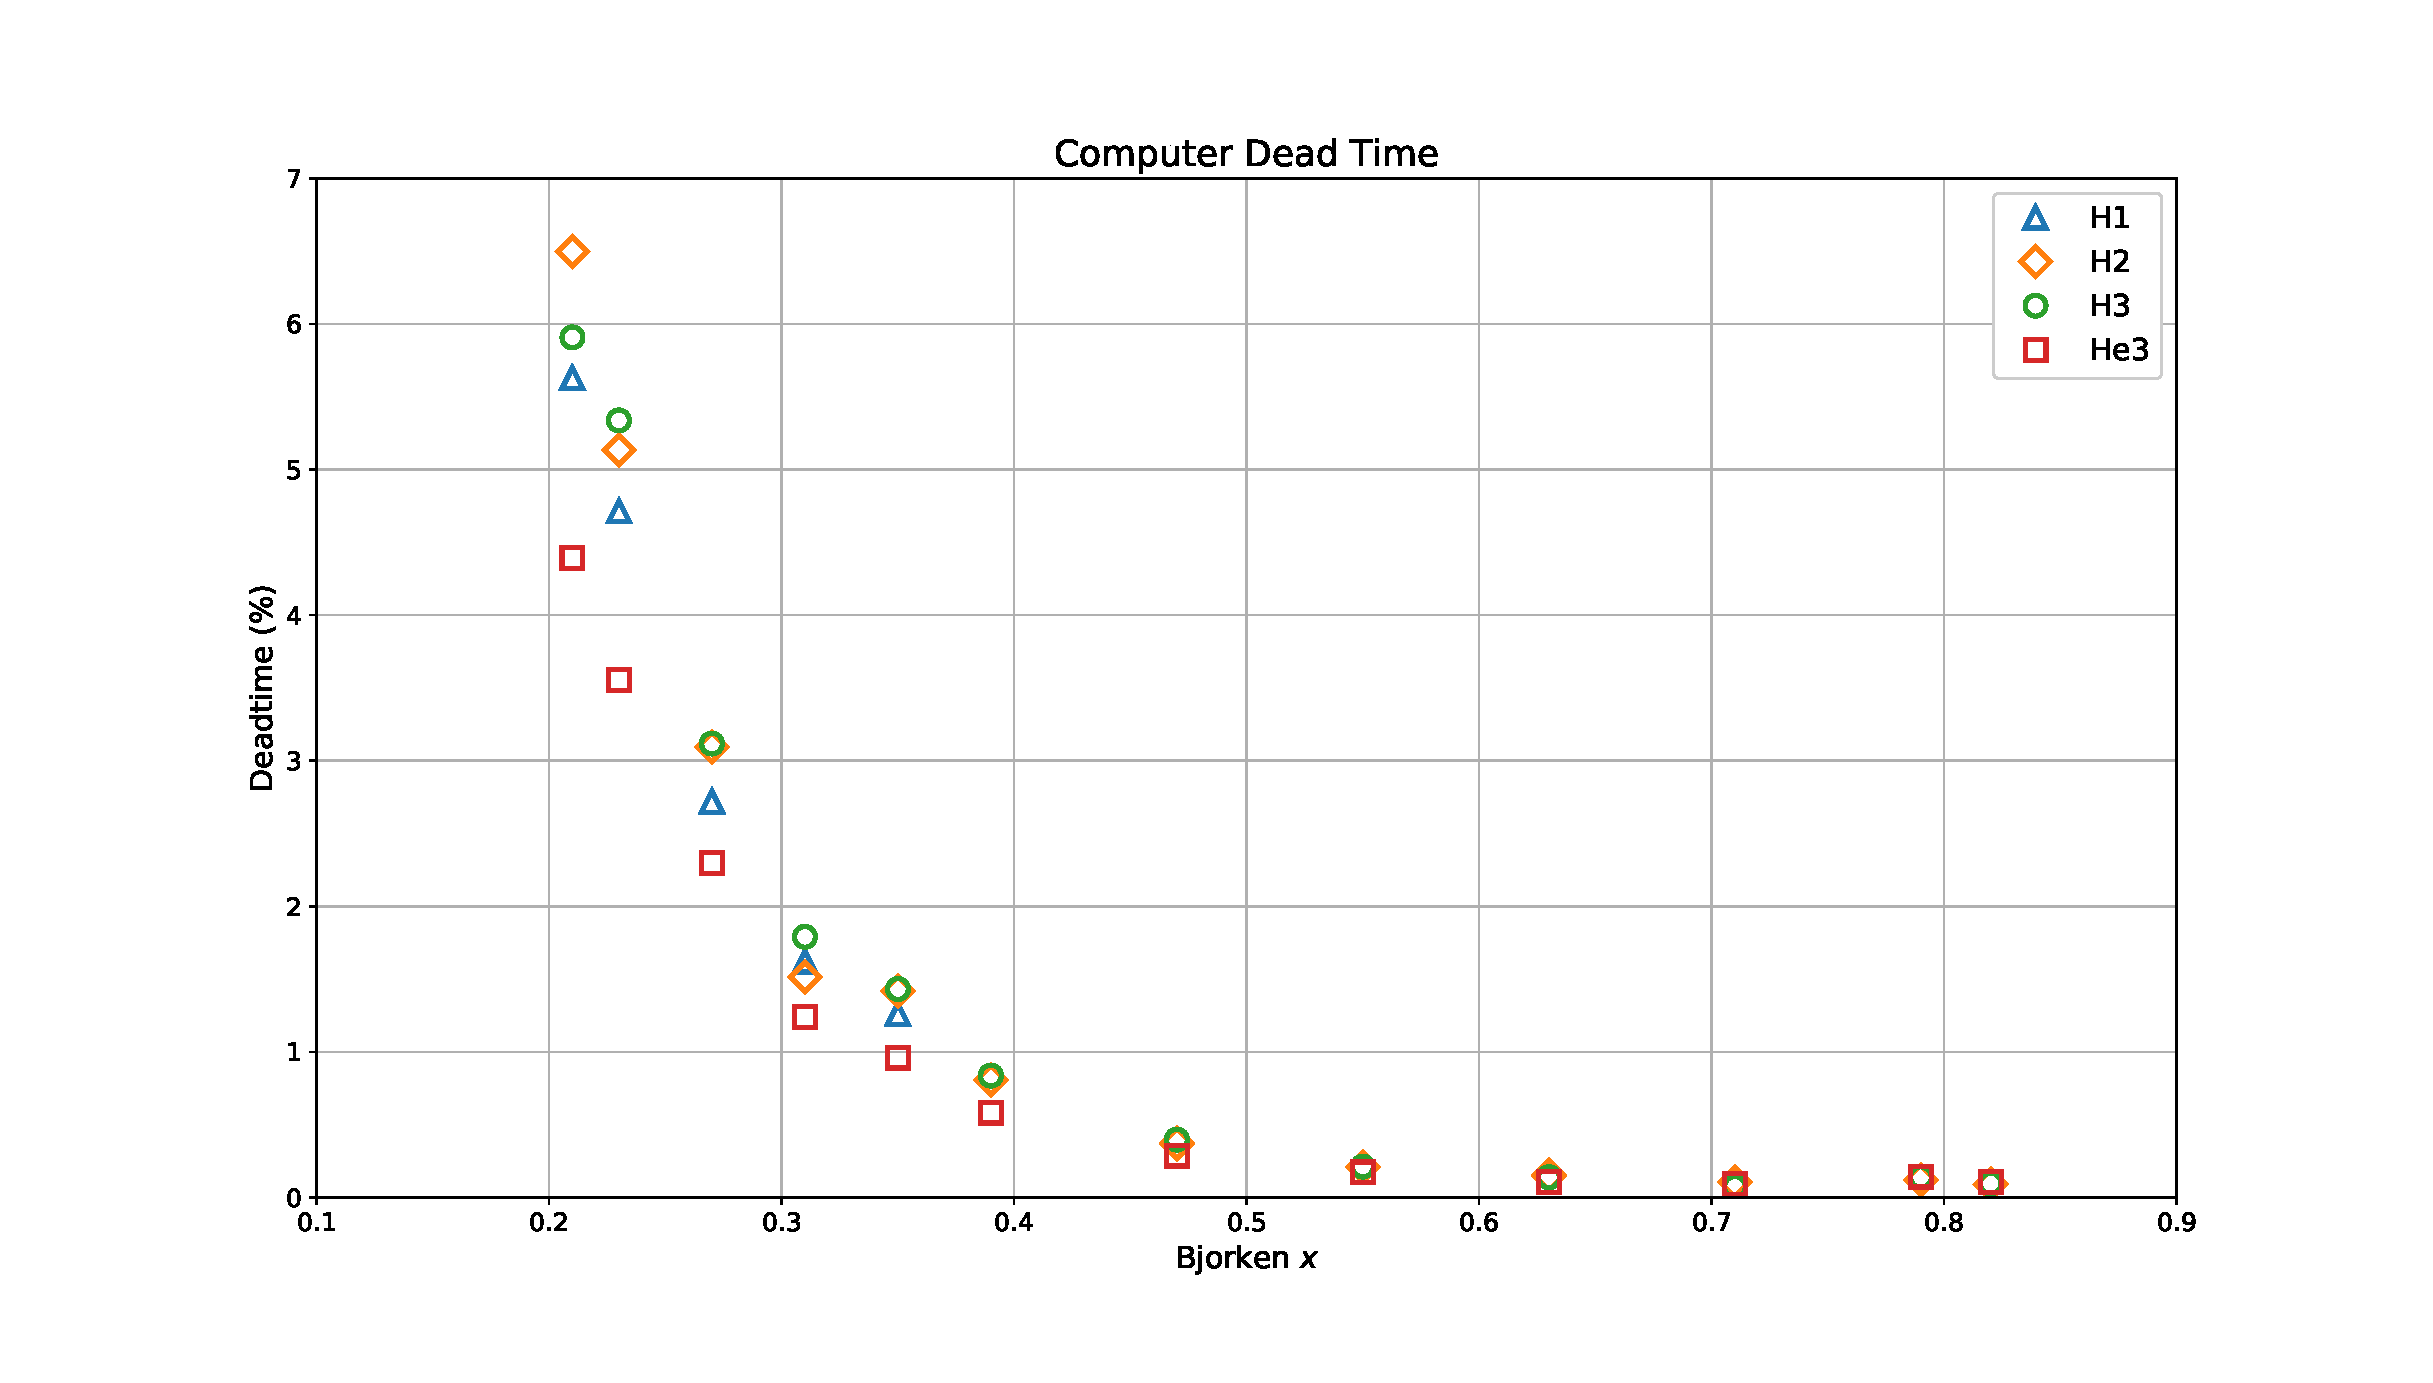
\includegraphics[width=\textwidth]{./analysis/fig/deadtime.eps}
	\caption{This plot shows the average computer deadtime in each kinematic (plotted at the central $x$ of the kinematic).}
	\label{fig:deadtime}
\end{figure}

\subsection{Target Boiling}
\label{sec:boiling}

When the beam is incident on the target, it deposits heat into the gas. This causes a density fluctuation of the gas referred to as ``target boiling''. The target does not actually boil, however that is the standard nomenclature for a density fluctuation in a gas target. When the density of the target changes, it changes the effective target thickness as seen by the beam. When the target thickness changes, there is a changed number of scattering centers which will lead to a change in the number of electrons recorded. Specifically, heating will decrease the target density which will decrease the number of scattered electrons.

The density changes are a function of the current on the target. Each run is taken at a single current so that the correction can be applied run by run. The correction is approximately linear for small deviations in current. A study of the effect during beam ramping found that the density settles very quickly. This means that so long as we cut events that occur with the beam off, it is unnecessary to take into account the beam ramping when correcting for this effect.

To determine the correction, a dedicated set of runs was taken with the Left HRS spectrometer at $16.8\degree$ and 3.1 GeV. At this kinematic, several data runs were recorded with varying current between them. Each of these runs were analyzed with the standard data cuts to determine the yield. This allows for the yield to be determined as a function of beam current.

Now that the yields have been determined as a function of beam current, they can be plotted and fit. The data is fit with a quadratic polynomial. This fit is constrained to require no correction (a correction factor of 1) at zero current. This is because the density must be the nominal fill density when there is no beam heating.

%Accidentally wrote a redundant paragraph
%Each run was recorded at a single nominal beam current. If there was a significant change in the current of the beam, the run was stopped and a new run was started. The target density correction is not linear with the beam current, so it is critical that each run have a very small range of beam current. Beam trips can be safely ignored because the density of the target reaches an equilibrium very quickly upon the beam reaching the set current. 

During analysis the average current is calculated for a run (ignoring beam trips). The average current is then used to calculate the target density correction with the fit function. The correction is then applied on a run-by-run basis by multiplying the number of scattering centers by this correction factor (or equivalently dividing the yield by the correction factor). Figure \ref{fig:boilcor} shows the correction factors for each target.\cite{boiling}

\begin{figure}
	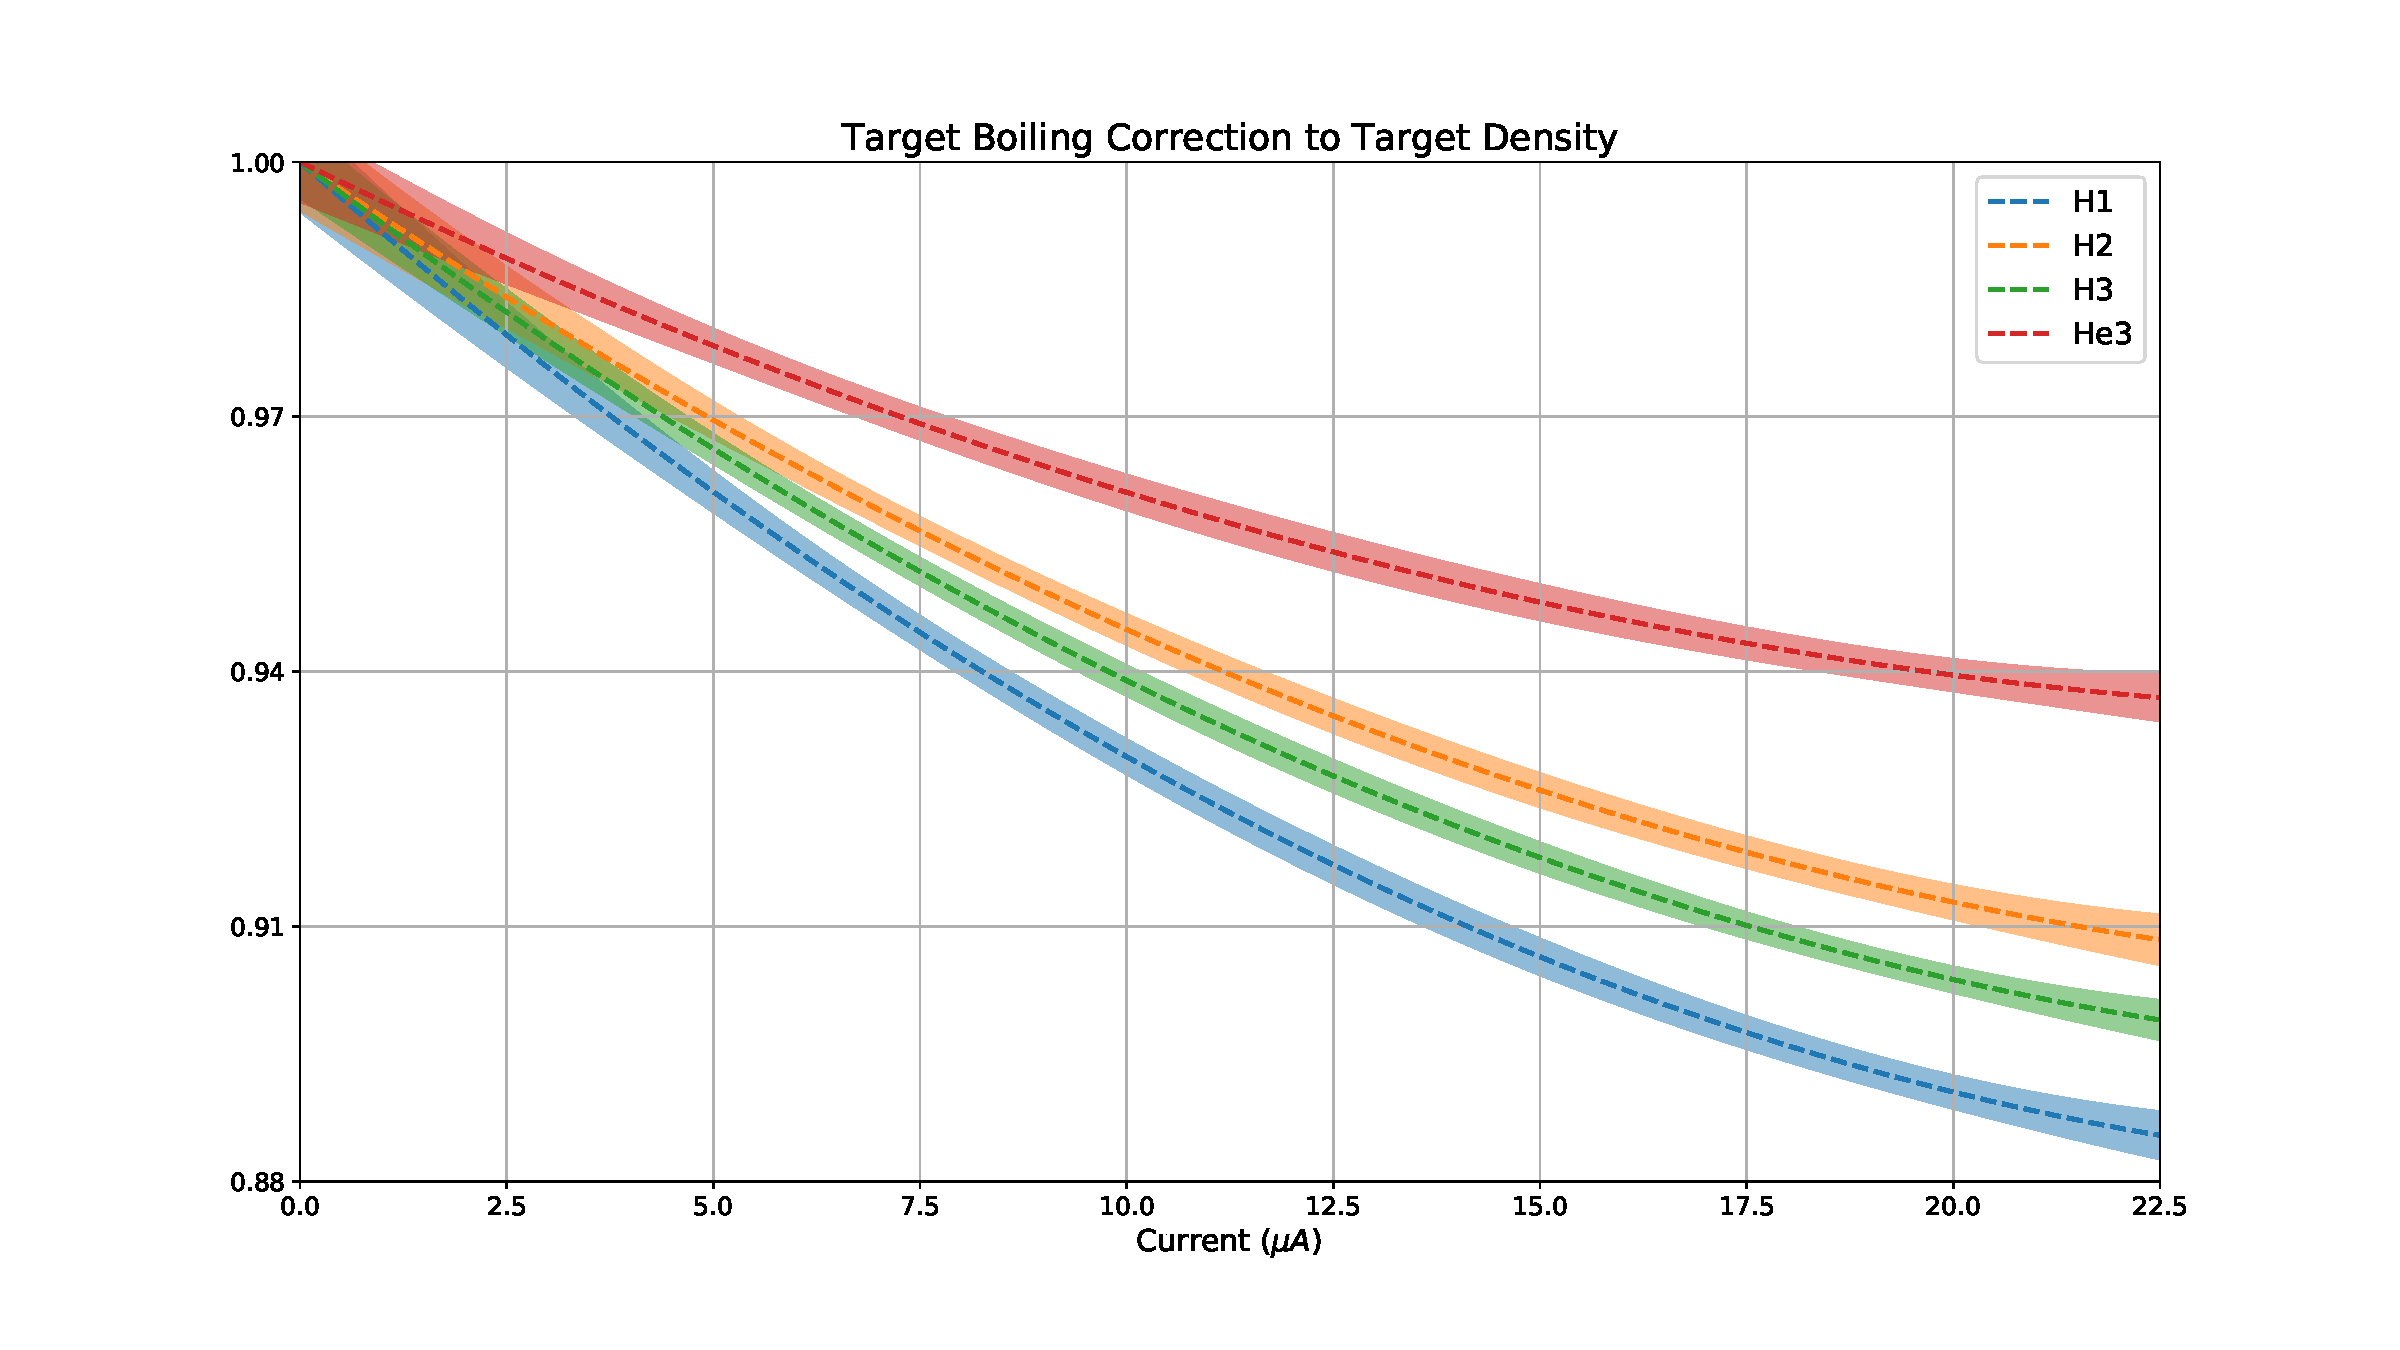
\includegraphics[width=\textwidth]{./analysis/fig/boil_cor.pdf}
	\caption{This plot shows the multiplicative correction to the target density due to beam heating. The correction is dependent on the beam current. The uncertainty band is plotted around each curve.}
	\label{fig:boilcor}
\end{figure}

%\begin{figure}
%	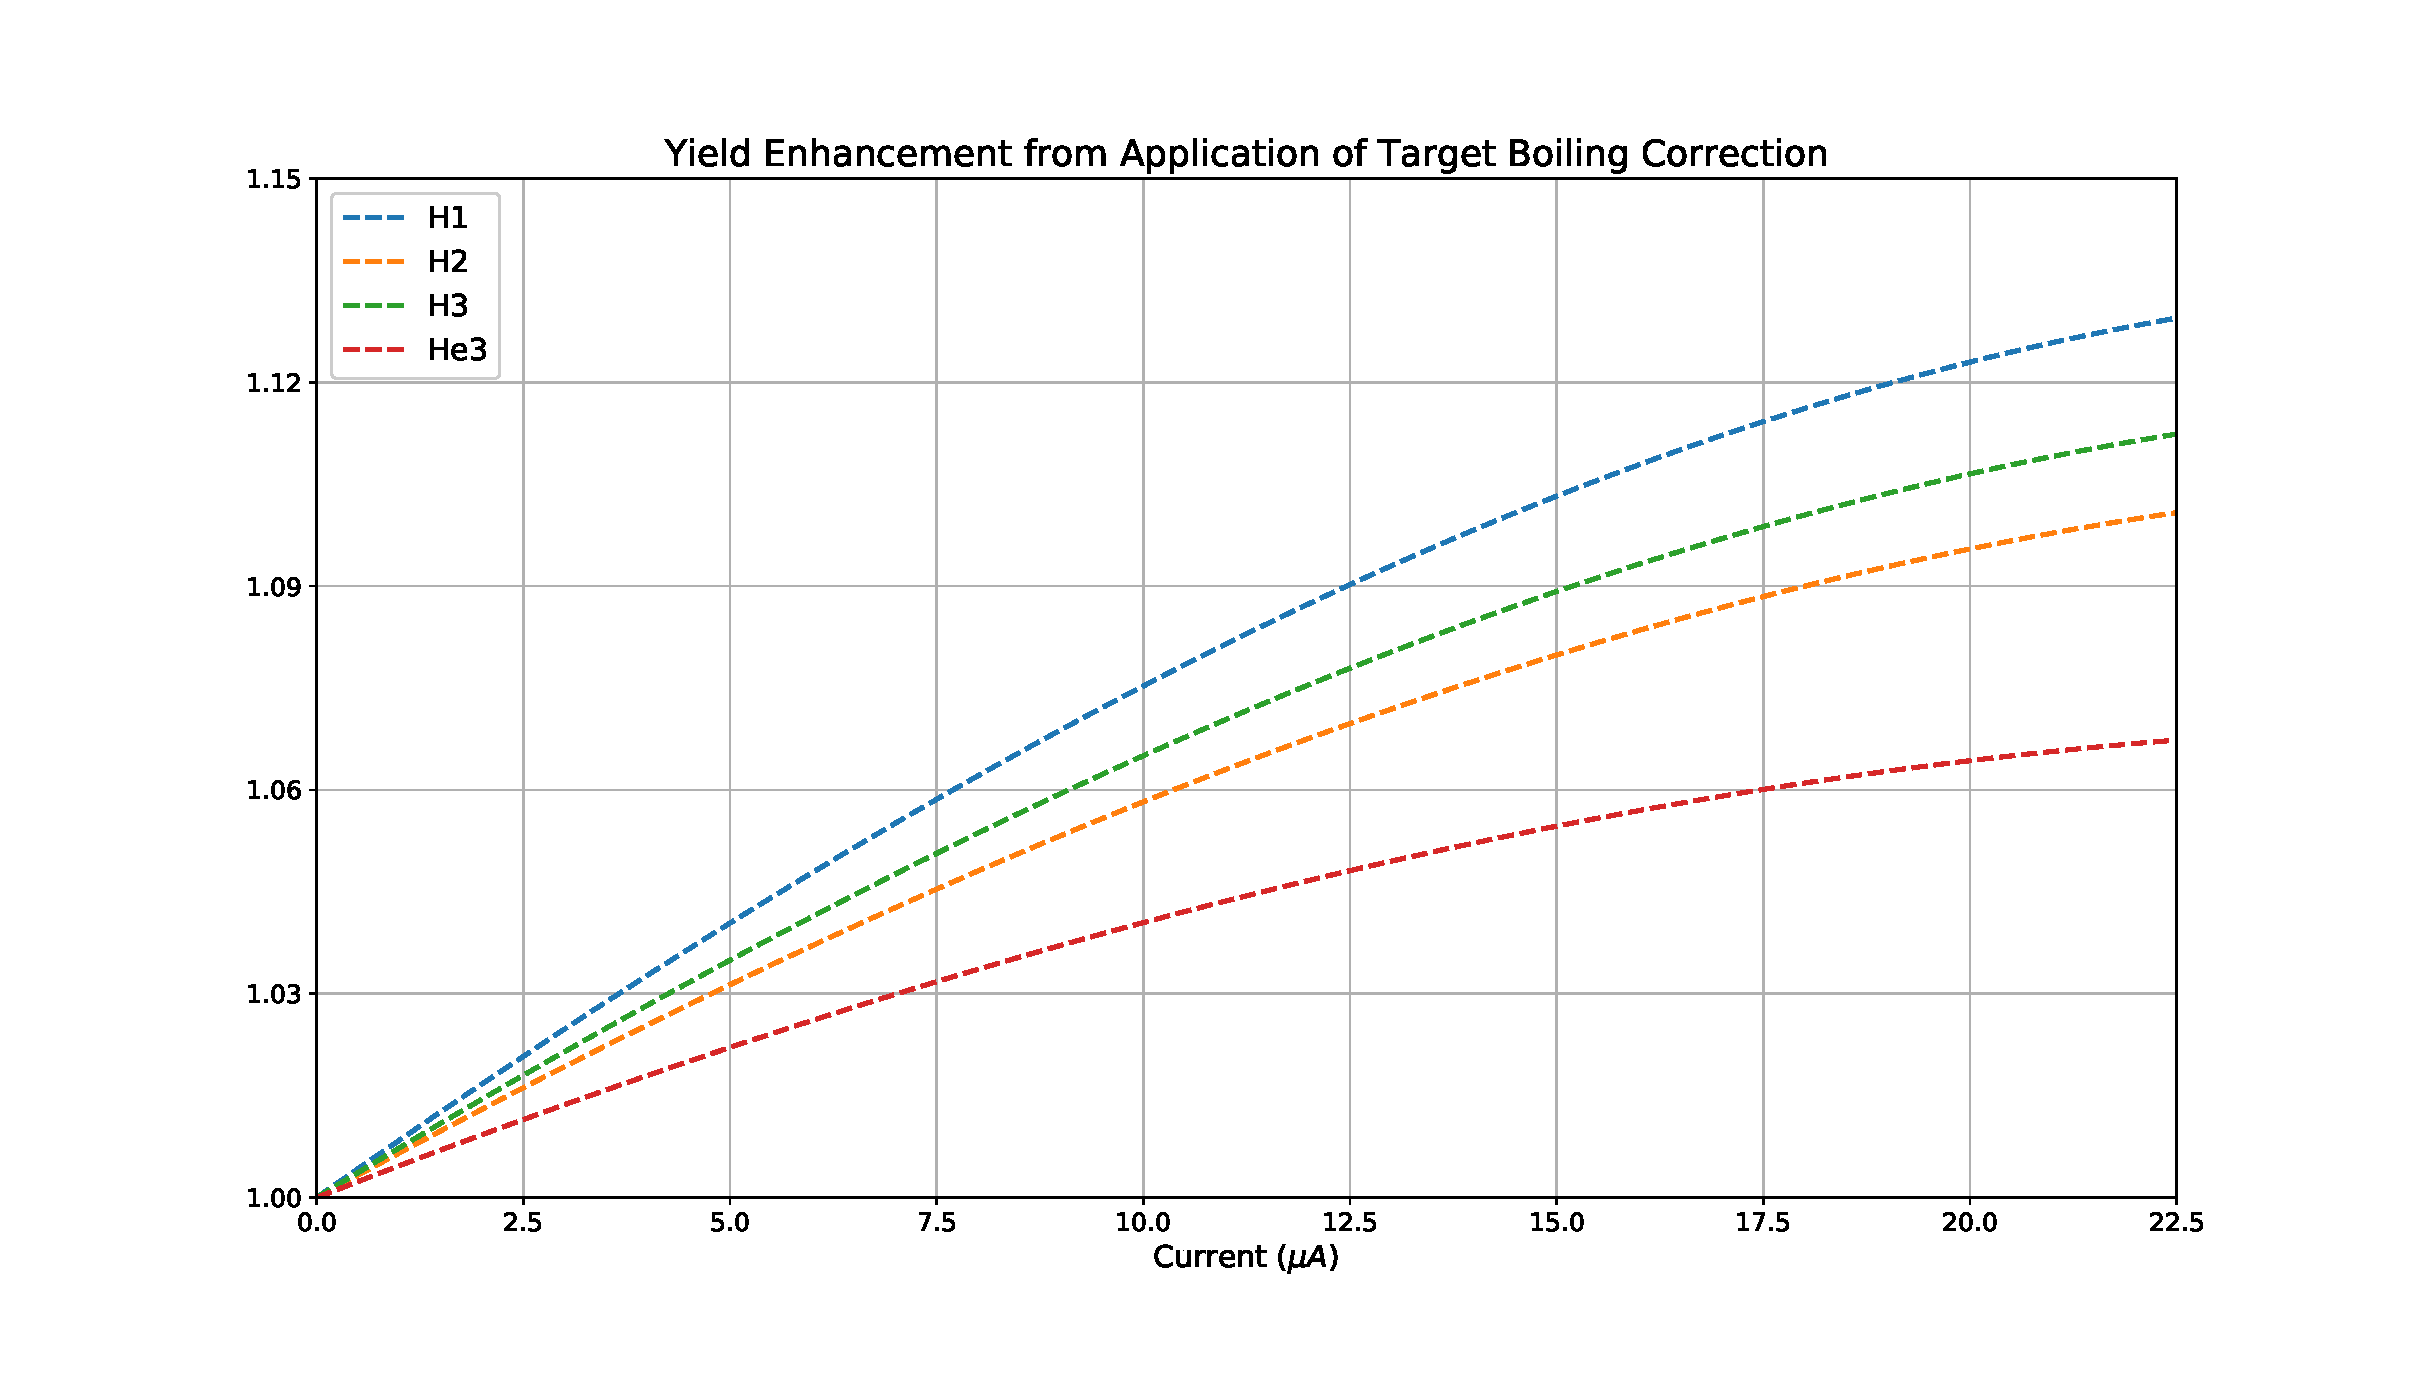
\includegraphics[width=\textwidth]{./analysis/fig/boil_yield_cor.eps}
%	\caption{Target density corrections cause a multiplicative enhancement to the yield}
%	\label{fig:boilyieldcor}
%\end{figure}

The uncertainty from this correction is calculated using the covariance matrix from the fit to the data. This uncertainty, like the correction, is applied on a run-by-run basis using the average current from the run. When all runs in a kinematic are combined, these uncertainties are summed linearly rather than in quadrature. This is because the uncertainties from the correction are completely correlated to each other. In a given kinematic, the combined uncertainty due to target boiling is approximately between $0.2$-$0.3\%$.

\subsection{Target Endcap Contamination}
\label{sec:ecc}

The gas targets used in this experiment are housed in aluminum cells as described in Section \ref{sec:gas_cell}. The thickness of the aluminum greatly exceeds the thickness of the gas and will contribute background that can survive the cuts placed on the data. By quantifying this contribution, the events that originate from the cell endcaps can be subtracted from the final results.

To determine this contribution, the empty cell is used. The empty cell, being an exact replica of the gas target cells with a vacuum inside, allows us to approximately isolate the contribution of the cell walls to the data. The empty cell and the target being studied are compared by calculating the yields on a kinematic-by-kinematic basis and normalizing them by charge and endcap thickness.

The normalization to the endcaps for each target must be done in two parts. This is because each endcap is not the same thickness. When calculating the yield for a target, it is assumed that any contamination upstream (downstream) of the center of the target must originate from the upstream (downstream) endcap. The two halves are then combined to arrive at the endcap thickness normalized yield. This yield calculation only has livetime corrections applied. All cuts are applied except for target length, which is adjusted to only include events upstream (downstream) of the center of the target.

The data for the target being studied and the normalized empty target are then binned in Bjorken $x$. Dividing the empty cell data by the gas target data then gives an approximation of the fractional contribution of the cell walls to the electron data. As this correction is applied to the final results, the contamination corrections for the targets are divided by each other to create the correction to the target ratios. These results are then fit with the functional form $1\pm e^{Ax+B}$. The choice of adding or subtracting the exponential is done by determining if the correction is greater or smaller than 1. The fit function and the covariance matrix of the fit are used to apply the correction to the final results as well as determine the uncertainty contribution of this correction. The uncertainty from this correction varies from $0.05$-$0.075\%$.

\begin{figure}
	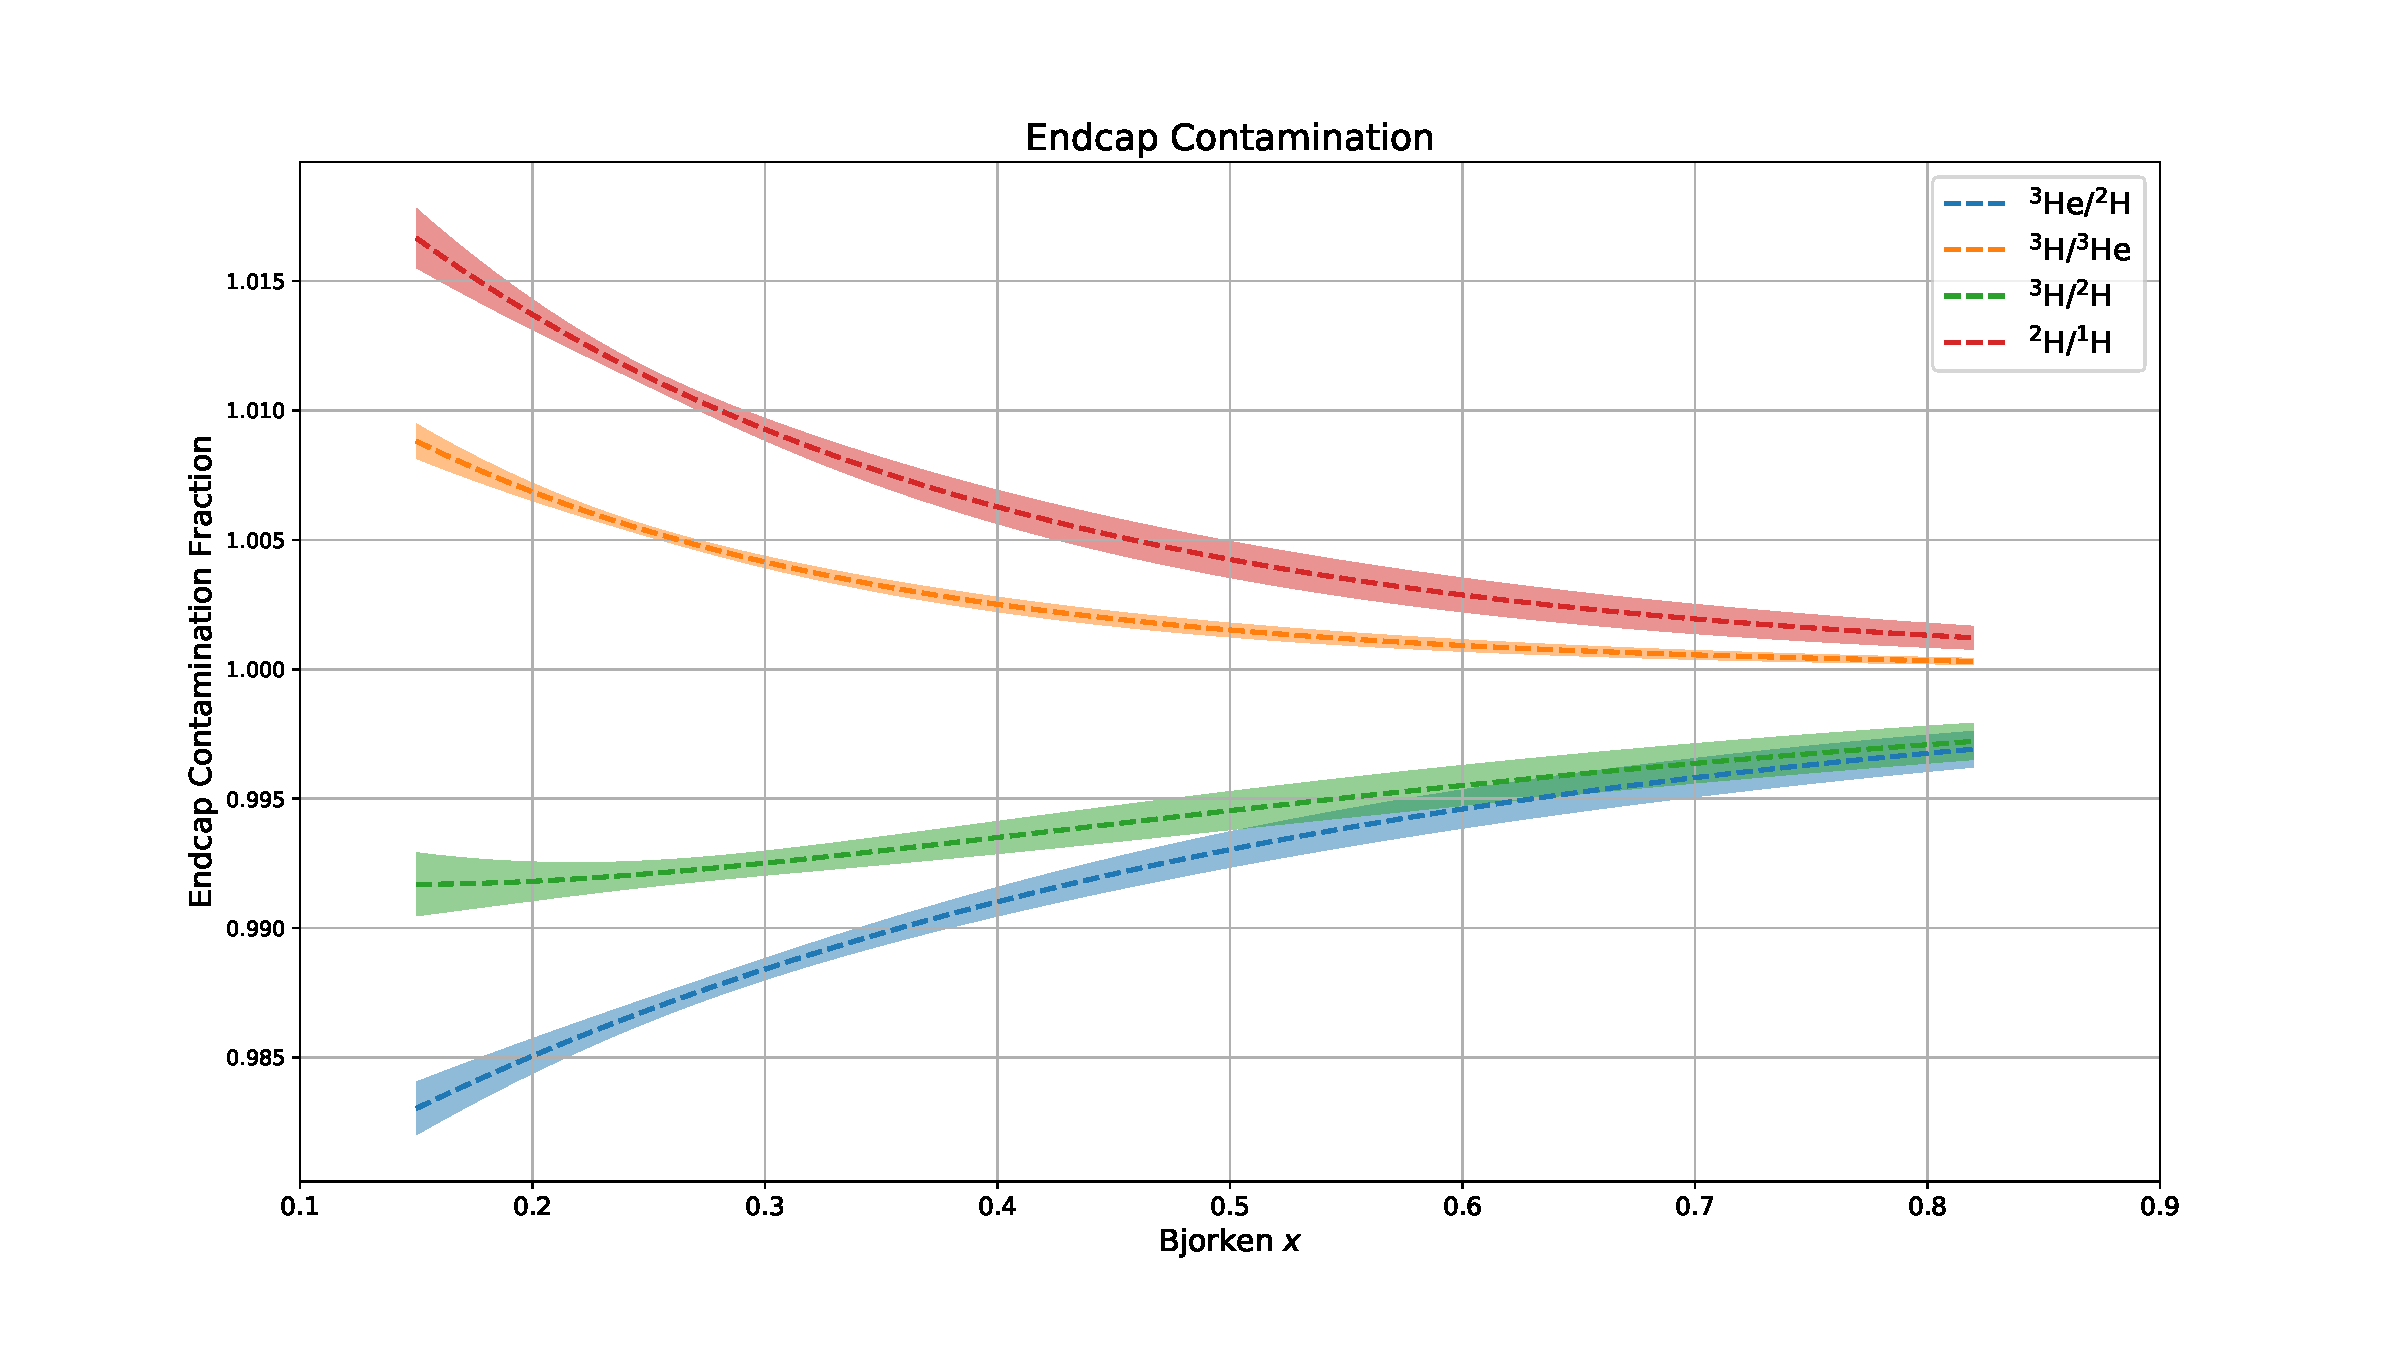
\includegraphics[width=\textwidth]{./analysis/fig/ECC.pdf}
	\caption{This plot shows the Endcap Contamination factor applied to each ratio studied MARATHON. The uncertainty band is plotted around each curve.}
	\label{fig:deadtime}
\end{figure}

\subsection{Charge Symmetric Background Subtraction}

As an inclusive scattering experiment, we are particularly susceptible to background from charge symmetric processes from the target. That is events which involved the production of both an electron and a positron, rather than the electron simply scattering. The primary source of this is $\pi^0$ decay. To study this, the polarity of the LHRS was reversed so that positively charge particles are directed into the detectors rather than negatively charged particles. With this setting, a number of runs were taken in kinematics 0 through 5. These runs were taken with all targets, just as the electron data was taken. This allows for a measurement of the positron yield which corresponds to a measure of the charge symmetric background.

This measurement allows us to determine the proportion of electrons that originated from pair production. Applying the same cuts and as the electron data allows us to determine the charge normalized positron yield. Unlike in the electron analysis, it was noted that there was significant pion contamination in the positron data. This pion contamination had to be subtracted in order to get an accurate calculation of the positron yield. This is achieved by fitting the main pion peak and the subtracting the tail of the fit which survives the cuts applied from the positron data.

The charge normalized positron yields over these kinematics are then combined (using the same methods as the electron yield) and binned in Bjorken $x$. This was then divided by the charge normalized electron yield. This is a fractional measure of the charge normalized background contamination. The ratio is then fit with an exponential of the form $e^{Ax + B}$, where $A$ and $B$ are the fit parameters. These fits are shown in in Figure \ref{fig:positrons}.

This correction is applied to the final yield ratio results. Both the numerator and denominator must have the charge symmetric background subtracted. Each target yield in the ratio is scaled by $\left(1 - e^{Ax + B}\right)$. For each bin, the fit is calculated at the bin center. The covariance matrix of the fit is used to calculate the uncertainty from this correction. The uncertainty varies from approximately $0.06\%$ at low $x$ to $.002\%$ at high $x$.

\begin{figure}
	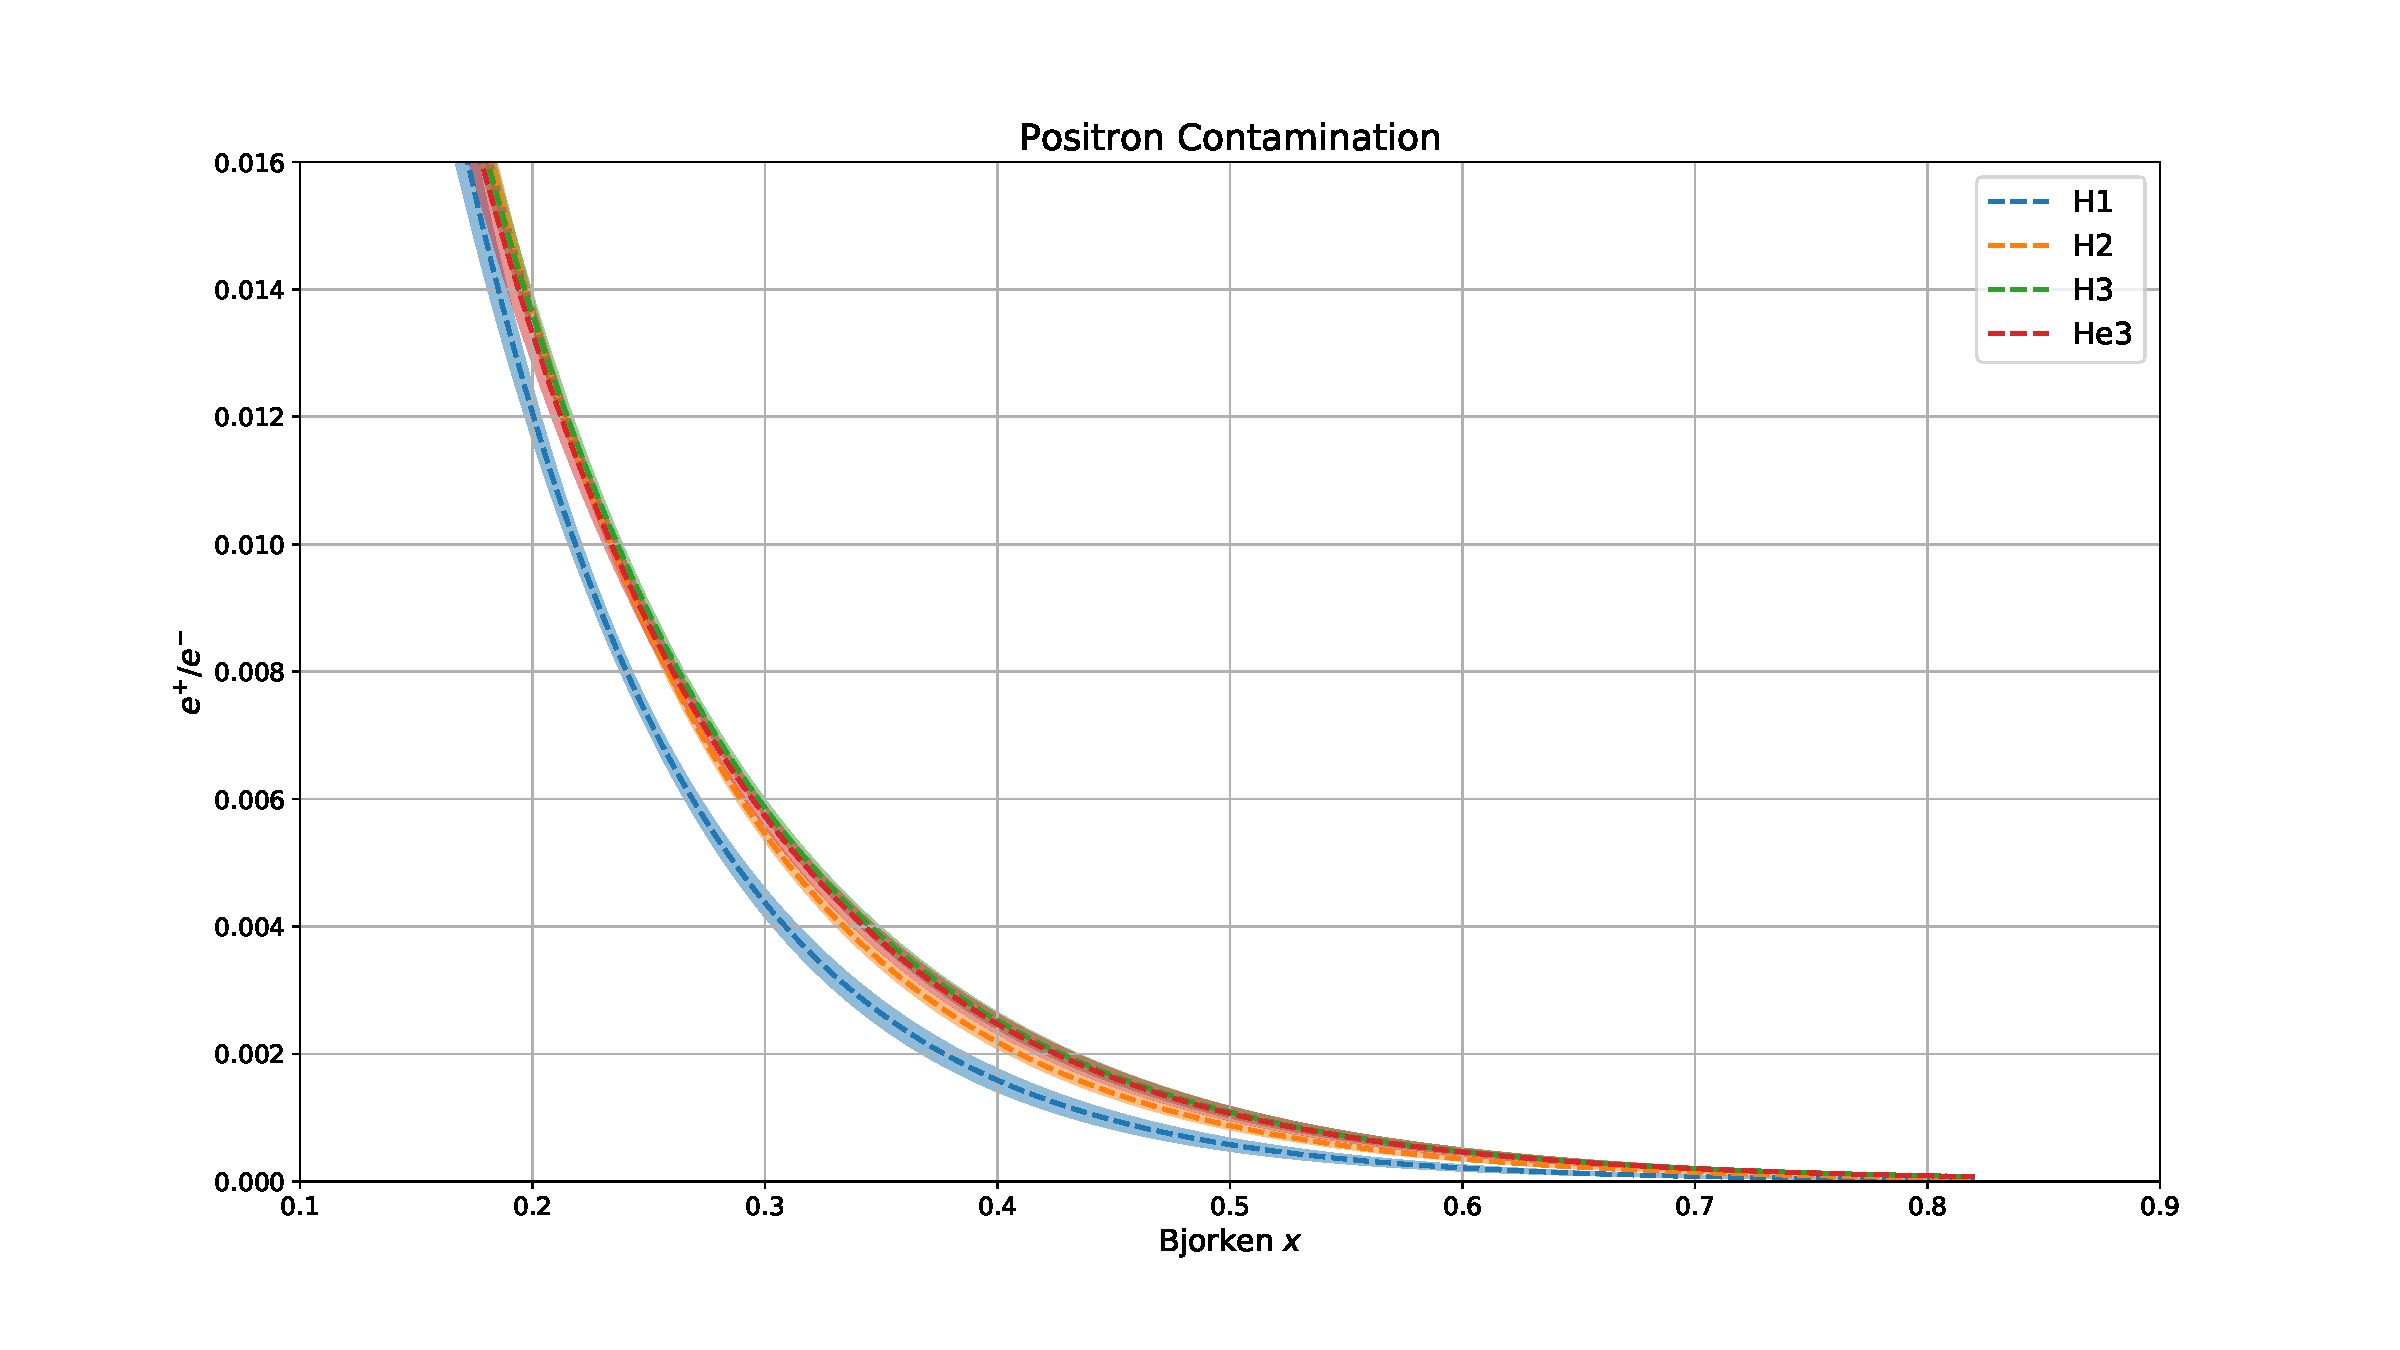
\includegraphics[width=\textwidth]{./analysis/fig/positrons.pdf}
	\caption{This plot shows the charge symmetric background correction to each target studied in MARATHON. The uncertainty band is plotted around each curve.}
	\label{fig:positrons}
\end{figure}

\subsection{Coulomb Corrections}

Corrections must be made for the effect of the charge of the target on the scattered electron. This interaction causes the $Q^2$ of the event to shift to an effective $Q^2$ value, $Q^2_{\rm eff}$. This conversion is done with the equation
\begin{equation}
	Q^2_{\rm eff} = Q^2 \left(1 + \frac{3Z\alpha\hbar c}{2RE}\right)^{2}.
\end{equation}
In this equation $R$ is the hard-sphere equivalent radius of the nucleus which is defined as $R=\left[\left(\nicefrac{5}{3}\right) \langle r^{2}\rangle\right]^{\nicefrac{1}{2}}$ where $\langle r^2\rangle$ is the root-mean-squared radius of the nucleus.\cite{coulomb}

Using $x=\frac{Q^2}{2M\nu}$, it is clear that a shift in $Q^2$ will result in a proportional shift in $x$. Using a model cross-section, the cross section is calculated at both the nominal $x$ and at $x_{\rm eff}$. As the results have been bin centered, this calculation uses a nominal $x$ at the center of the bin. This will lead to the correction
\begin{equation}
	\sigma_{\textrm{Coulomb Corrected}} = \sigma_{\rm data} \frac{\sigma_{\rm model}\left(x_{\rm eff}\right)}{\sigma_{\rm model}\left(x\right)}.
\end{equation}

This correction is applied to the final ratio and each target in the ratio must be corrected. The ratio is multiplied by the correction to the numerator and divided by the correction to the denominator. The covariance matrix of the fit to the model is used to determine the uncertainty of this correction. The uncertainty from the Coulomb Correction is approximately $0.15$-$0.2\%$.

\begin{figure}
	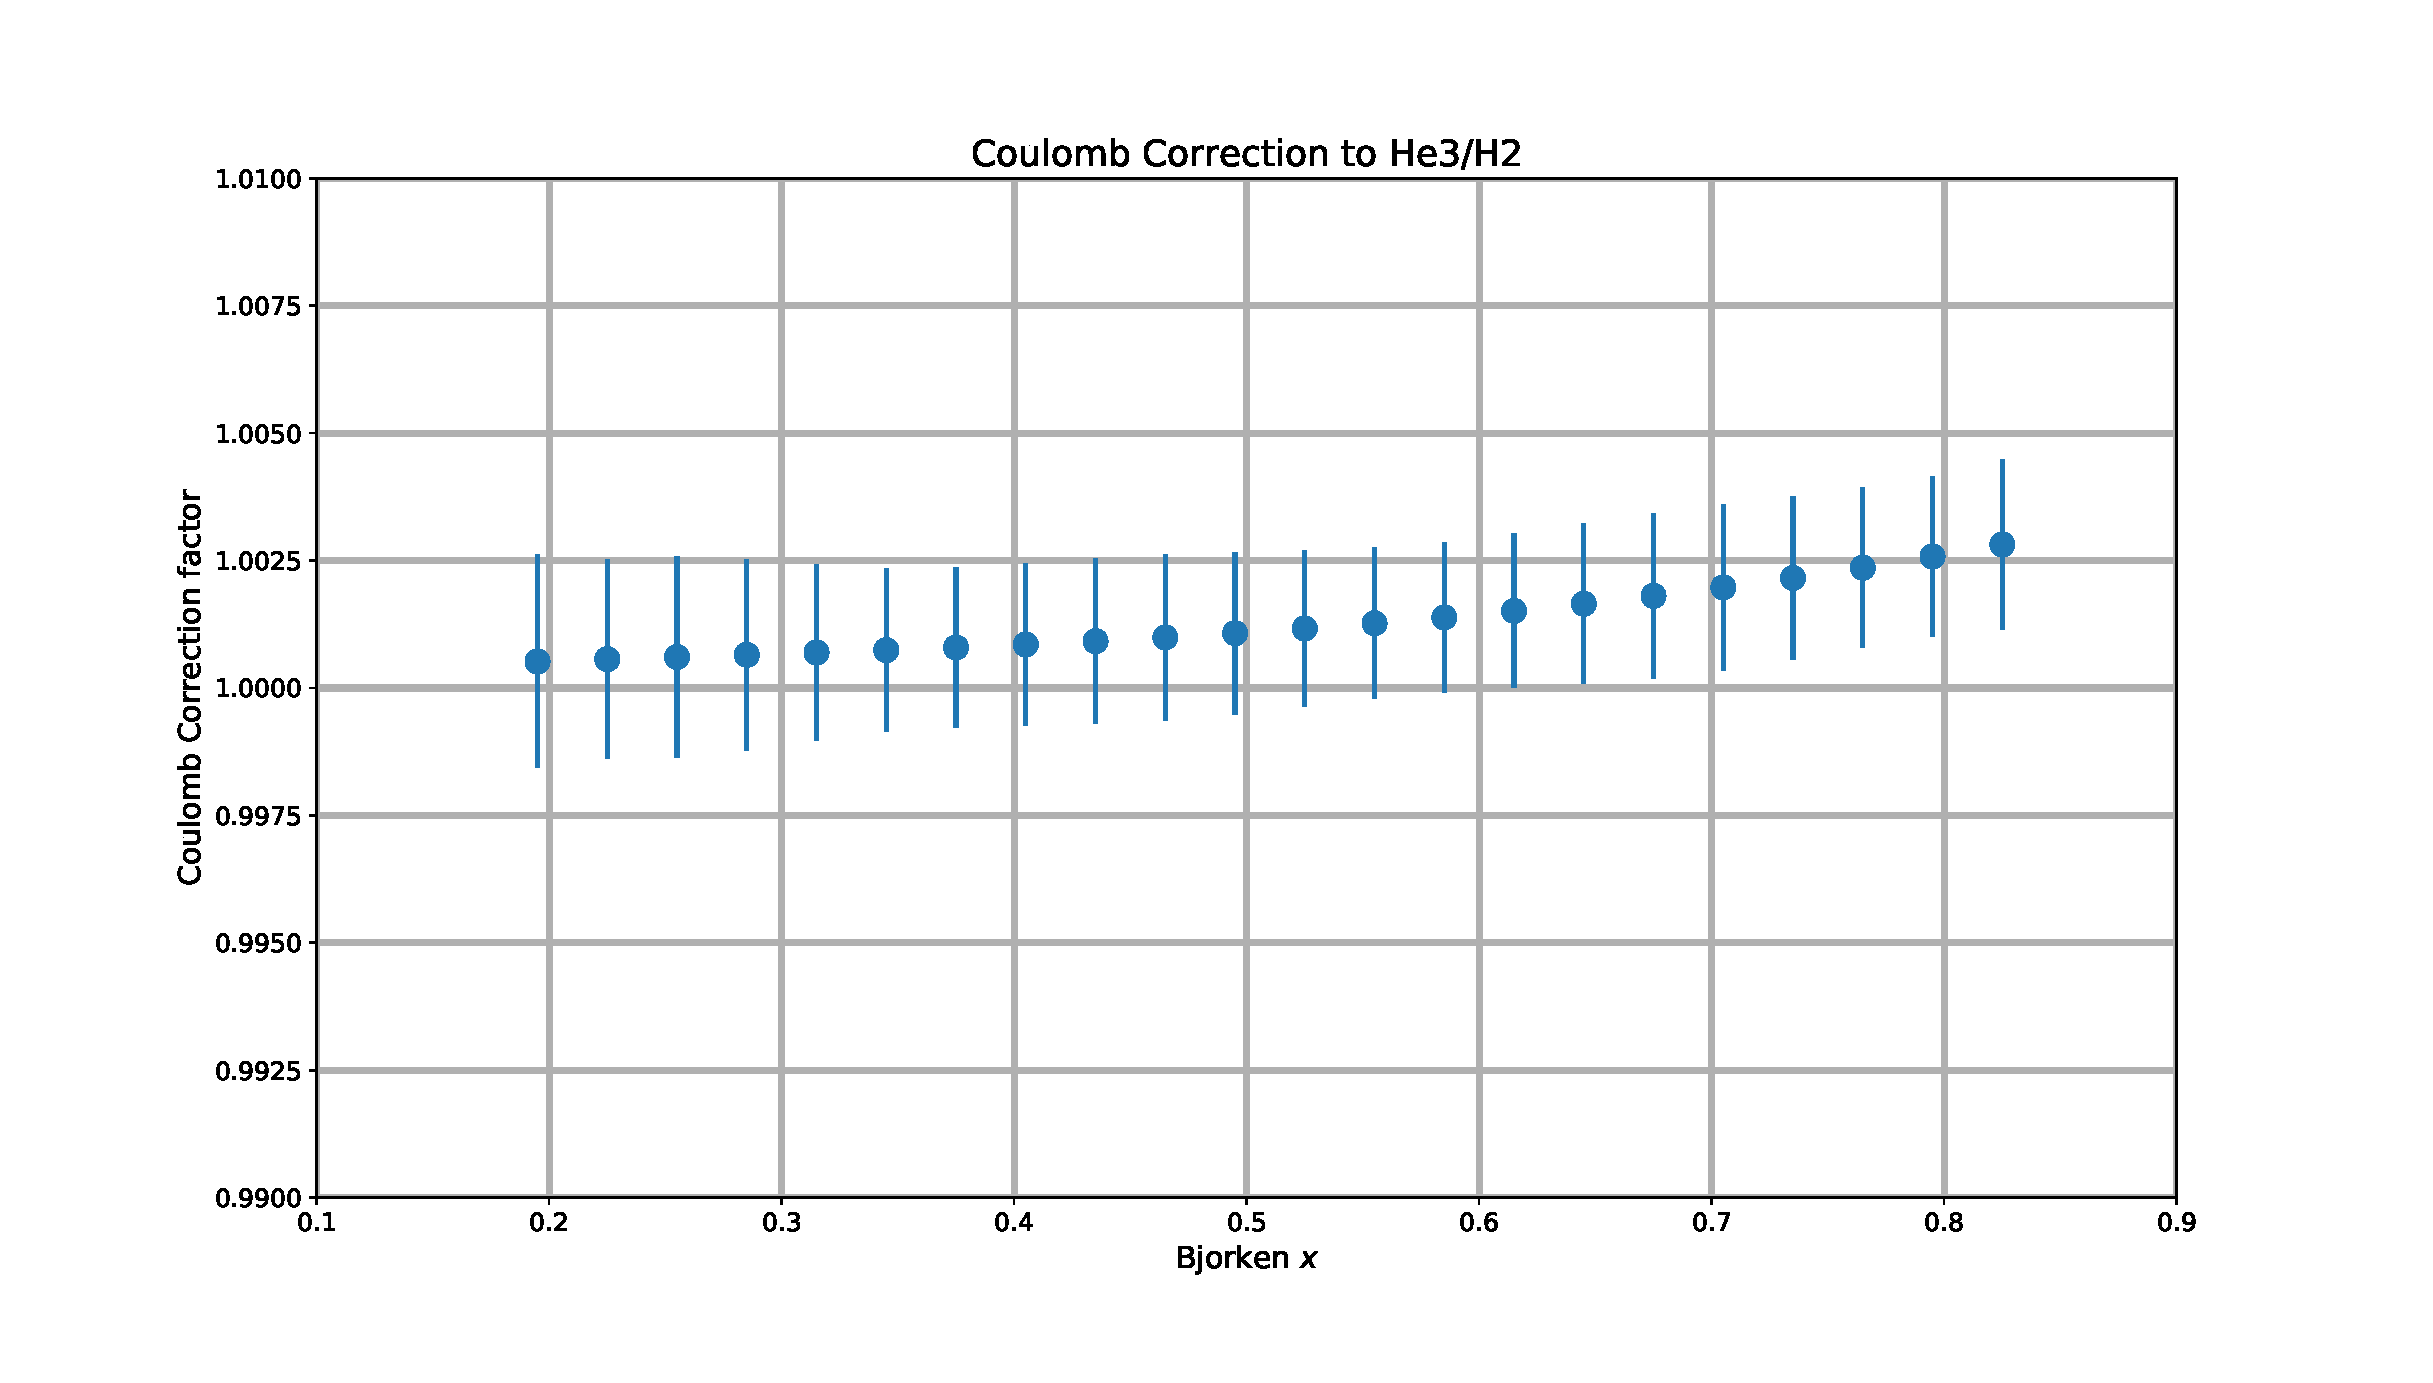
\includegraphics[width=\textwidth]{./analysis/fig/cc.eps}
	\caption{This plot shows the Coulomb Correction values to the \nicefrac{$^3$He}{$^2$H} ratio by bin with the uncertainty on the correction.}
\end{figure}

\subsection{Bin Centering Corrections}

The cross-section over the width of a bin is not constant. This means that the measurement does not correspond with the true cross section at the center of the bin. Rather, because the data is effectively ``sampled'' over the bin the measured value corresponds to the expectation value of the cross-section within the bin. If the results are to be reported at the bin center, the data must be corrected to the bin center.

Using a model that matches the shape of our data well, the location of the measurement within the bin can be calculated. This is done by calculating the expectation value of the model within that bin and determining the $x$ value corresponding to this value. The expectation value is given by
\begin{equation}
	\langle f_{\rm measured}\rangle = \frac{1}{\Delta x}\int_{x_{\rm low}}^{x_{\rm high}} f\left( x \right) dx,
\end{equation}
where $f$ is a function representing the chosen model. In practice, the $x$ value does not need to be calculated if the data will be reported at the bin center. Rather, the correction is simply the ratio of the model at the bin center. This is written as
\begin{equation}
	\sigma_{\textrm{Bin Centered}} = \frac{f\left(x_{\textrm{Bin Center}}\right)}{\langle f_{\rm measured}\rangle} \sigma_{\rm measured}.
\end{equation}

This correction must be applied to both targets in the ratios. That is, the ratio must be multiplied by the correction to the numerator and divided by the correction to the denominator.\cite{wtsydp} The covariance matrix of the fit to the model is used to determine the uncertainty of this correction. The uncertainty from the Bin Centering Correction is approximately $0.3\%$.

\begin{figure}
	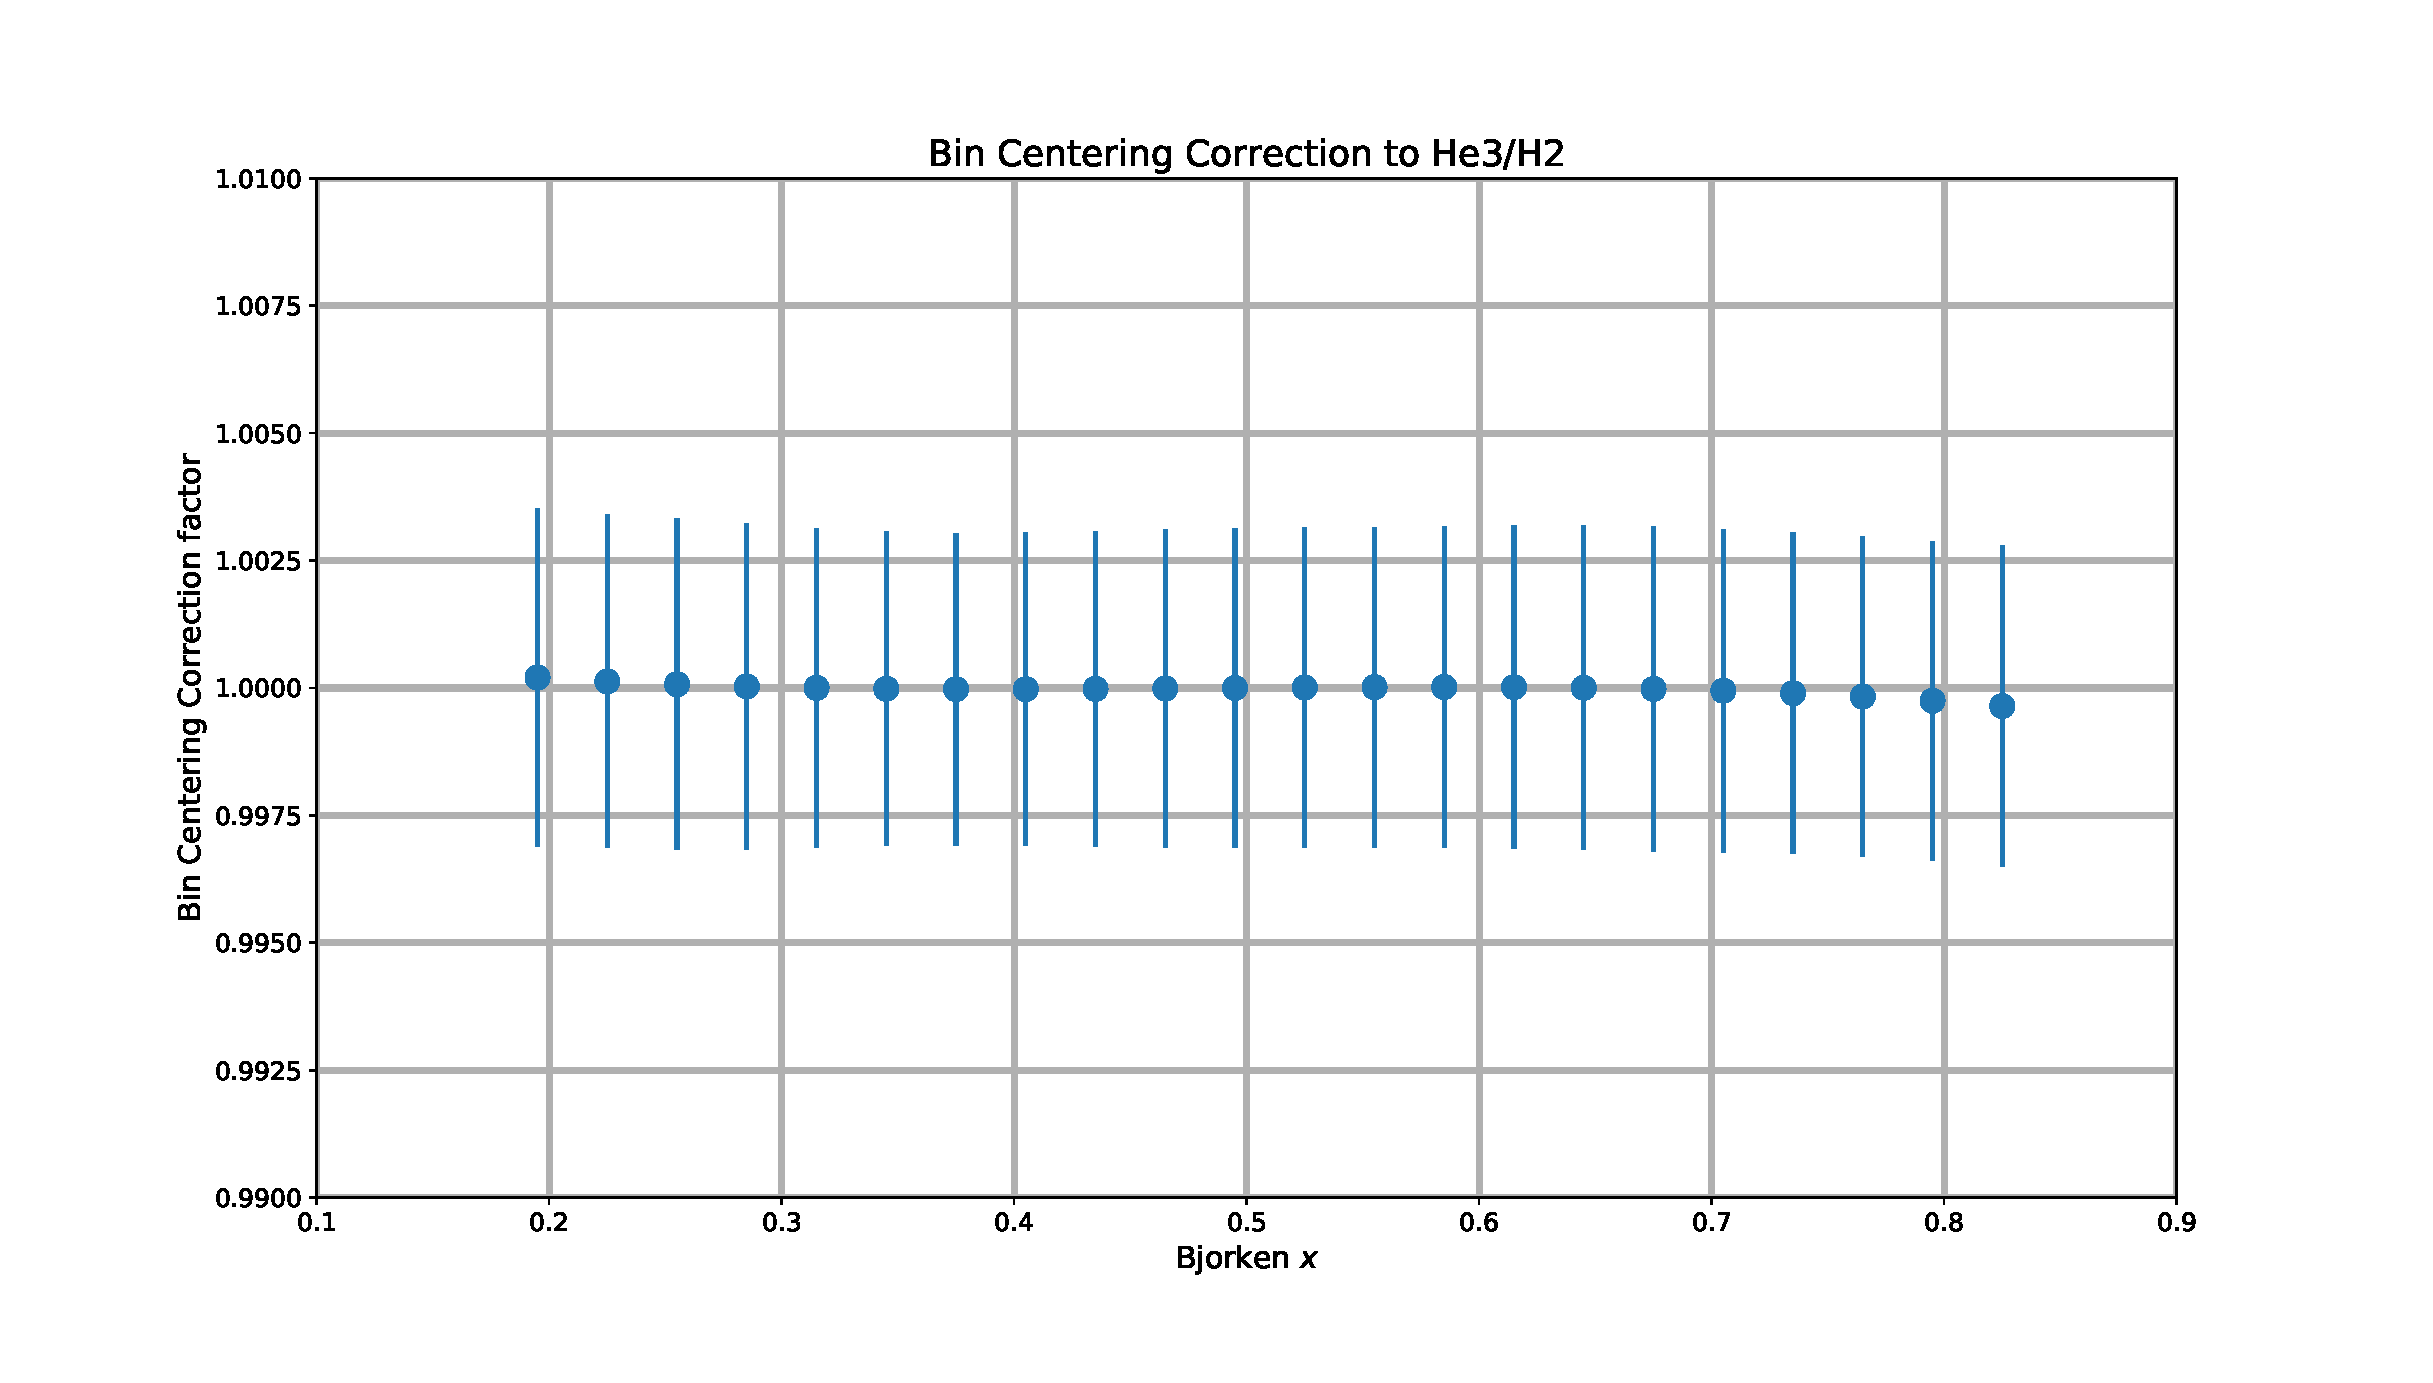
\includegraphics[width=\textwidth]{./analysis/fig/bcc.eps}
	\caption{This plot shows the Bin Centering Correction values to the \nicefrac{$^3$He}{$^2$H} ratio by bin with the uncertainty on the correction.}
\end{figure}

\subsection{Radiative Corrections}

The Deep Inelastic Cross Sections being studied are the Born approximation of a single-photon exchange. The Born approximation is the simplest interaction that can occur in which an electron enters, exchanges a photon with the parton, and then subsequently scatters. In this approximation, no other photons are exchanged or radiated. The measurement however, contains contributions from higher order processes that will increase the measured cross section. These processes include Bremsstrahlung, vertex corrections, and vacuum polarization. Bremsstrahlung is when the incoming or outgoing electrons radiate photons due to deceleration. Vertex corrections are the emission and subsequent reabsorbtion of a photon by the incoming and outgoing electron. Vacuum polarization is when the virtual photon exchanged between the electron and nucleon annihilates into a particle-antiparticle pair which then reannihilate back into a virtual photon. Using a model, these and higher order contributions can be corrected for and removed from the measurement.

The experiment used a software package called $\texttt{T2\_EXTERNALS}$ that calculates both the Born cross section and the radiated cross section for a given target at a kinematic set $(E,E^{\prime} ,\theta )$. For this analysis, the values used in the calculation correspond to the center of the bin being corrected. After the calculation is complete, the radiative correction is
\begin{equation}
	\textrm{RC} = \frac{\sigma^{\textrm{radiated}}_{\textrm{model}}}{\sigma^{\textrm{Born}}_{\textrm{model}}}.
\end{equation}

The uncertainty was determined by using different models of the radiative corrections. There was little difference between the models. Ultimately, the uncertainty due to radiative corrections was determined to be $0.5\%$ for all data points.

\begin{figure}
	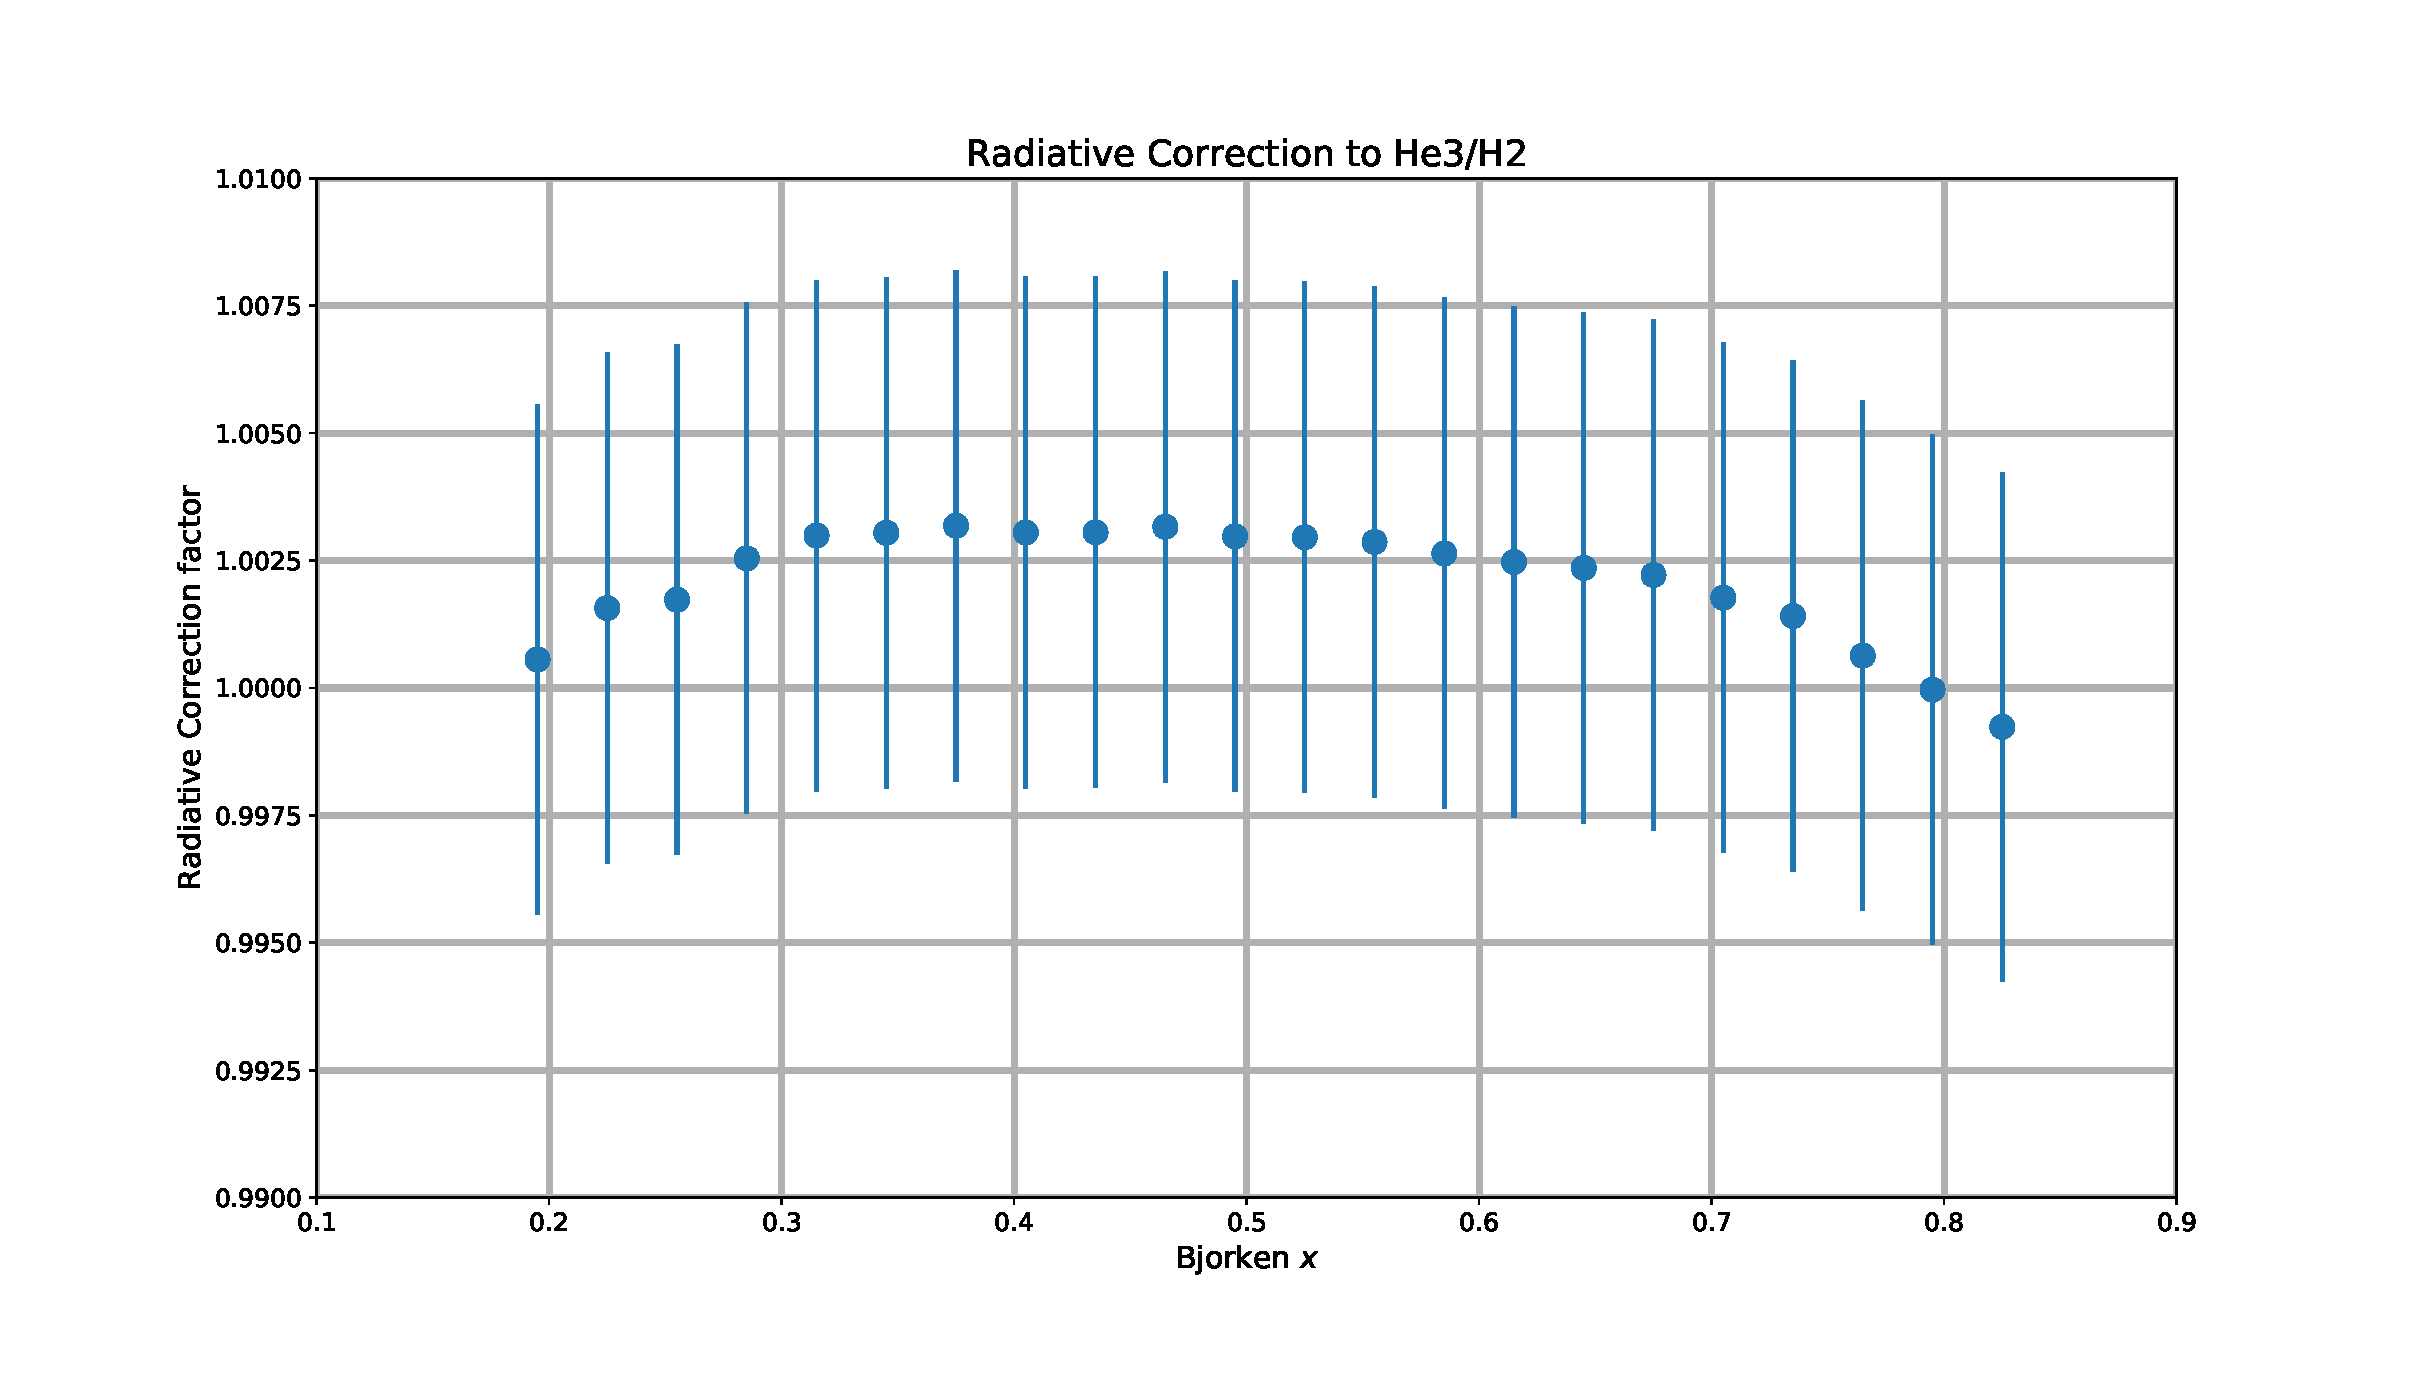
\includegraphics[width=\textwidth]{./analysis/fig/radcor.eps}
	\caption{This plot shows the Radiative Correction values to the \nicefrac{$^3$He}{$^2$H} ratio by bin with the $0.5\%$ uncertainty on each value.}
\end{figure}

\subsection{Isoscalar Corrections}
\label{sec:isocor}

When studying an EMC ratio, the strength of the EMC effect is typically defined using isoscalar nuclei, nuclei where the number of protons and the number of neutrons are equal. Helium-3 is not an isoscalar nucleus. To study the EMC effect, we ``correct'' this to create a fictional $A=3$, $Z=\nicefrac{3}{2}$ isoscalar nucleus. This correction uses $\nicefrac{F_2^n}{F_2^p}$ as extracted from the MARATHON $^3$H/$^3$He ratio to transform the proton excess into equal quantities of protons and neutrons. This correction is defined as
\begin{equation}
	\textrm{Isoscalar Correction} = \frac{\frac{1}{2}\left(1+\nicefrac{F_2^n}{F_2^p}\right)}{\frac{1}{A}\left(Z+\left(A-Z\right)\nicefrac{F_2^n}{F_2^p}\right)}
\end{equation}

The covariance matrix of the fit to the $\nicefrac{F_2^n}{F_2^p}$ data is used to determine the uncertainty of this correction. After the uncertainty is propagated, the uncertainty is between $0.36\%$ and $0.67\%$.

\begin{figure}
	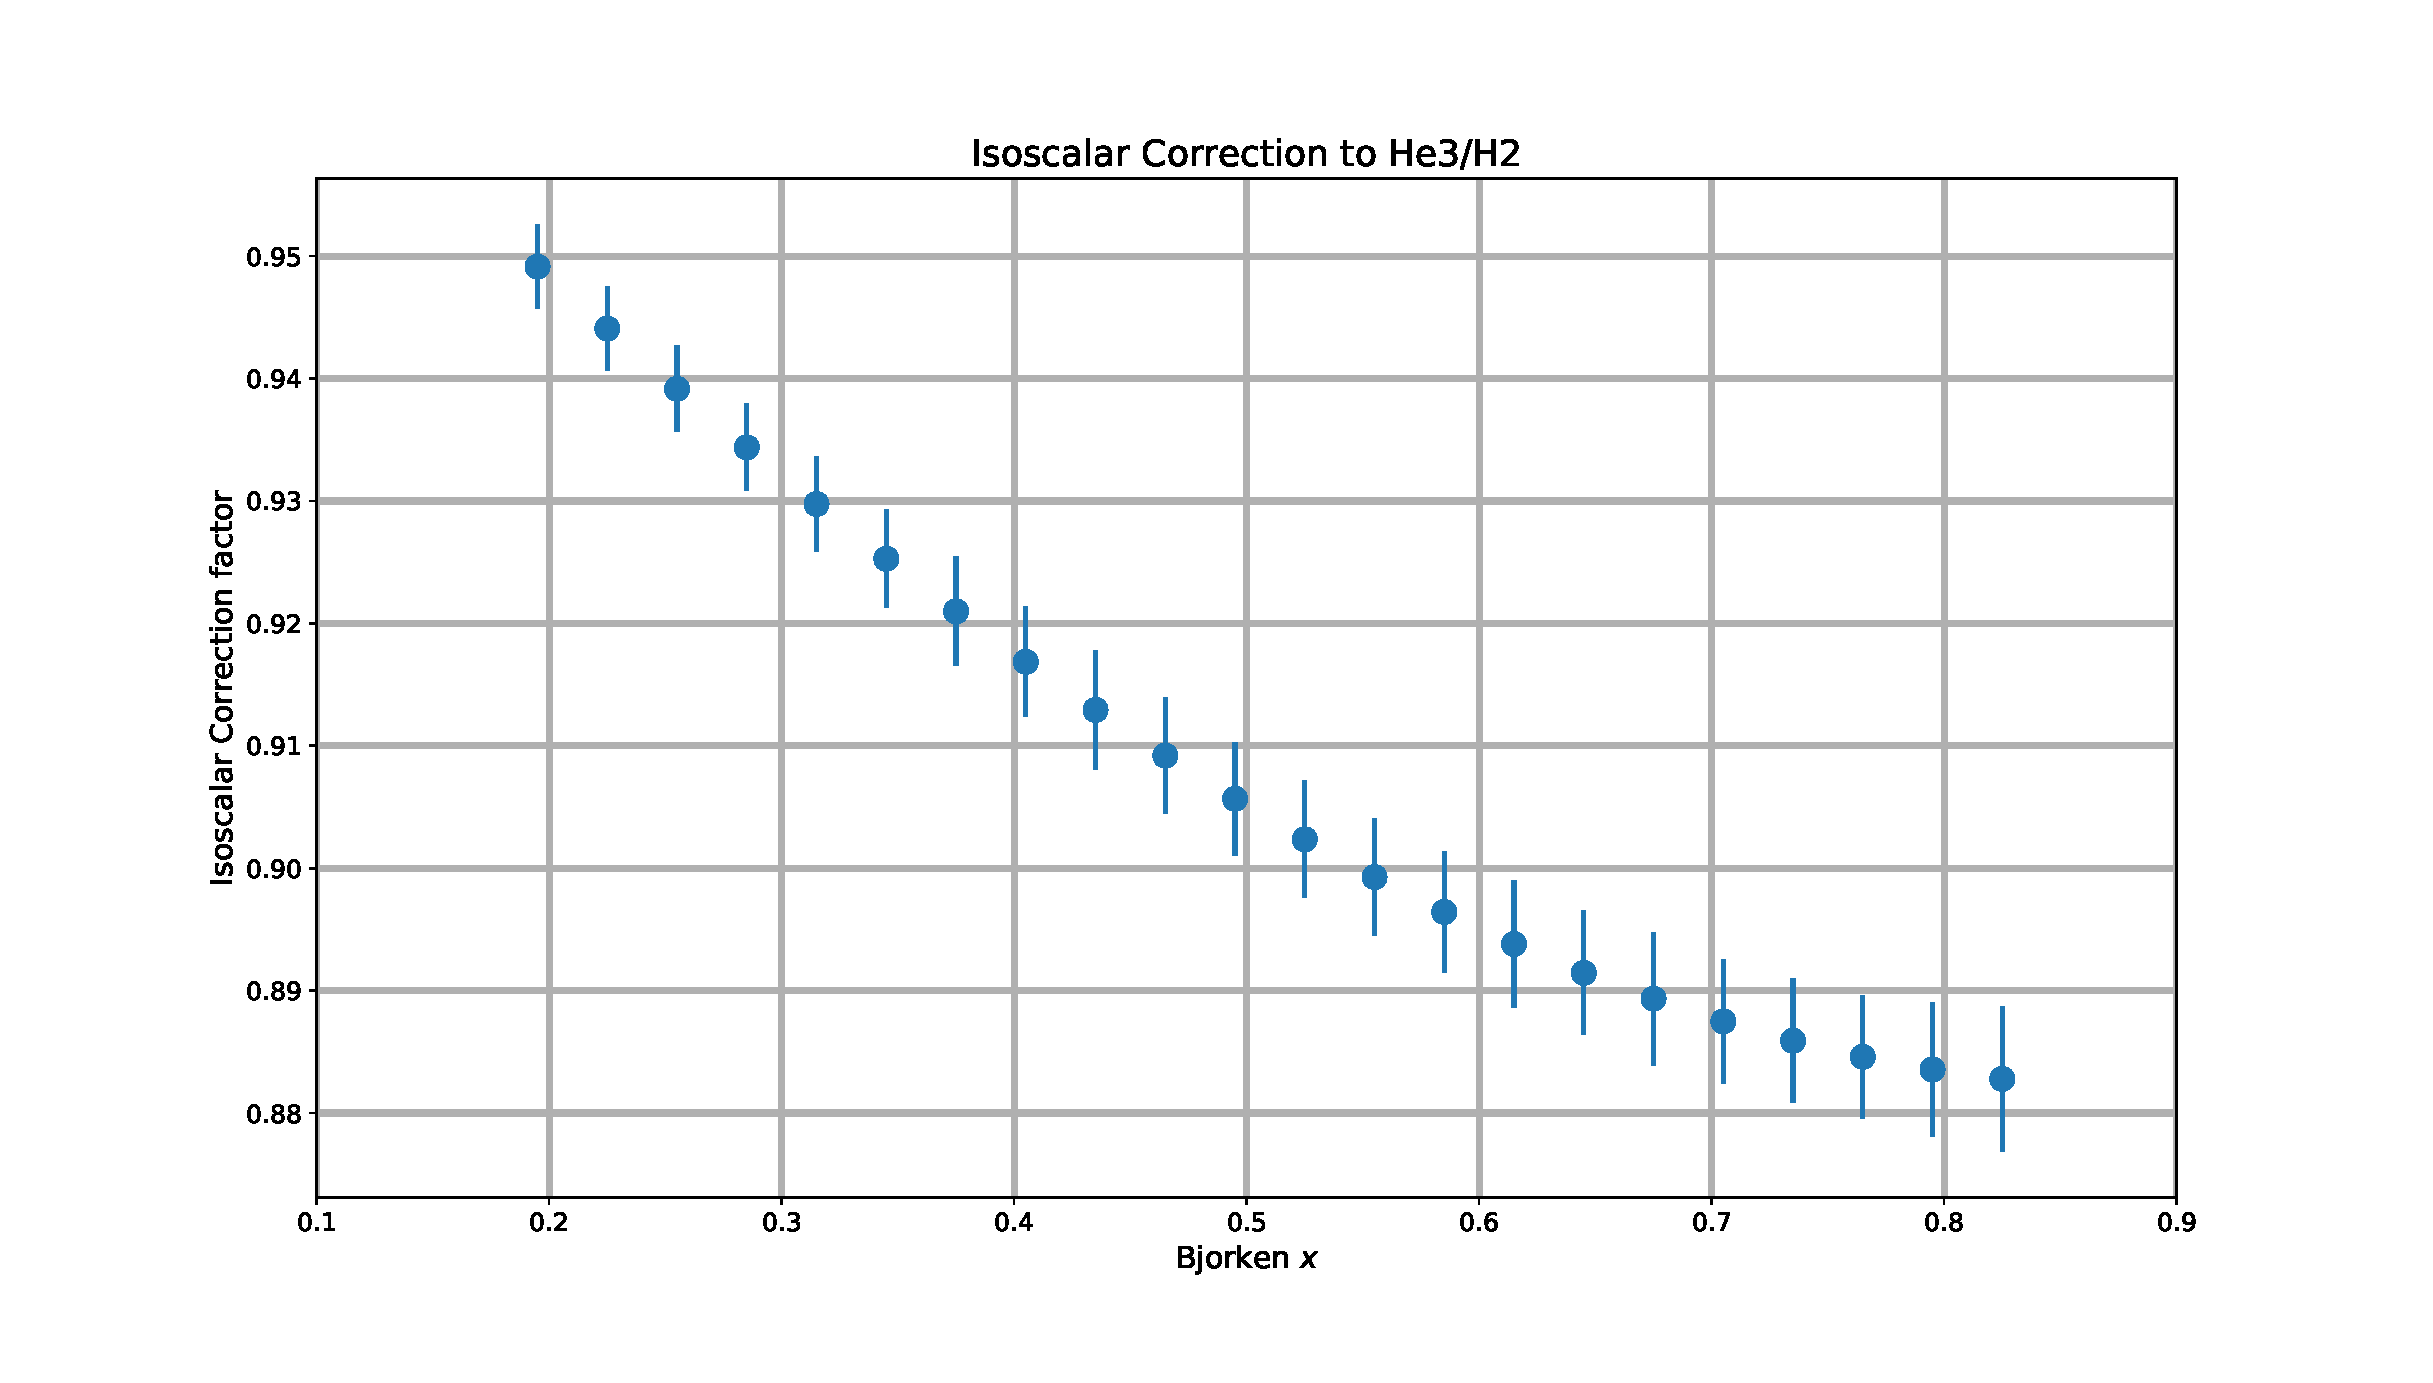
\includegraphics[width=\textwidth]{./analysis/fig/isocor.eps}
	\caption{This plot shows the Isoscalar Correction values to the \nicefrac{$^3$He}{$^2$H} ratio by bin with the uncertainty on the correction.}
\end{figure}


